\documentclass[a4paper,12pt,twoside,openright]{report}

\usepackage[a4paper]{geometry}
\usepackage{amssymb,amsmath,amsthm}
\usepackage{graphicx}
\usepackage{url}
\usepackage{hyperref}
\usepackage{enumitem}
\usepackage{epsfig}
\usepackage[italian]{babel}
\usepackage{setspace}
\usepackage{emptypage}
\usepackage{thesis}
\usepackage{parskip}
\usepackage{booktabs}
\usepackage[justification=centering]{caption}
\usepackage{nicematrix}
\usepackage[linesnumbered, ruled]{algorithm2e}
\usepackage[utf8]{inputenc}

% CUSTOM COMMANDS

\newcommand{\partitioned}[2]{#1\slash\!\!#2}  % partitioned set
\newcommand{\bigo}[0]{\mathcal{O}}            % big O notation

% THEOREMS ENVIRONMENTS

\newtheorem{theorem}{Teorema}[chapter]        % theorem
\newtheorem{definition}{Definizione}[chapter] % definition
\newtheorem{lemma}{Lemma}[chapter]            % lemma
\newtheorem{corollary}{Corollario}[theorem]    % corollary

% ALGORITHM ENVIRONMENT

\SetKwComment{Comment}{/* }{ */}  % comment style
\SetKwInOut{Input}{Parametri}     % input text
\SetKwInOut{Output}{Output}       % output text
\newenvironment{algo}[3]{
  \IncMargin{1.3em}
  \begin{algorithm}
    \SetAlgorithmName{Algoritmo}{}{}
    \DontPrintSemicolon
    \caption{#1}
    \vspace{0.1em}
    \Indmm\Indmm
    \Input{#2}
    \Output{#3}
    \Indpp\Indpp
    \vspace{0.1em}
}{
  \end{algorithm}
  \DecMargin{1.3em}
}

% DOCUMENT

\begin{document}
% \raggedbottom with this the last line of the page is not aligned with the bottom of the page

% FRONTPAGE

\title{Iperminimizzazione di automi a stati finiti deterministici}
\author{Andrea TINELLI}
\dept{Corso di Laurea in Informatica} 
\anno{2023 - 2024}
\matricola{941800}
\relatore{Prof. Giovanni PIGHIZZINI}

% i think that this is not needed, but i have to verify
% with the professor, to re-enable it: remove the comment
% from the next line and from the thesis.sty file
% \correlatore{nome COGNOME}

% BLANK PAGE

\beforepreface
\prefacesection{}
{\hfill {\sl Questa pagina è stata lasciata intenzionalmente vuota.}}

% PREFACE

\prefacesection{Prefazione}
Prefazione

% ORGANIZATION

\section{Organizzazione della tesi}
\label{organizzazione}
La tesi \`e organizzata come segue:
\begin{itemize}
  \item nel Capitolo 1 sono presentate le nozioni preliminari e necessarie alla comprensione dell'elaborato riguardanti la teoria degli automi;
  \item nel Capitolo 2 è presentato il problema dell'iperminimizzazione di automi a stati finiti deterministici;
\end{itemize}

% THANKS TO

\prefacesection{Ringraziamenti}
grazie a 
\afterpreface

% CHAPTER 1

\chapter{Nozioni preliminari}
\label{cap1}

La teoria degli automi è uno dei principali e più antichi campi dell'informatica teorica. In questo capitolo
ne vengono presentati i concetti fondamentali. Per un'esposizione più completa il lettore è rimandato a \cite{HMU06}.

\section{Alfabeti, parole e linguaggi}

Un \emph{alfabeto}, generalmente indicato con la lettera $\Sigma$, è un insieme finito di simboli,
entità astratte non definite formalmente cui esempi possono essere lettere e numeri.

Una \emph{parola} (o \emph{stringa}) è una sequenza finita di simboli giustapposti, in particolare, una parola su un alfabeto $\Sigma$
è una sequenza finita di simboli appartenenti a $\Sigma$.

La \emph{lunghezza di una parola} $w$, indicata con $|w|$, è il numero di simboli che la compongono.
Caso particolare è la parola vuota, a cui per convenzione si fa riferimento con la lettera $\varepsilon$,
composta da zero simboli ($|\varepsilon| = 0$).

Un possibile esempio di alfabeto è $\Sigma = \{0, 1\}$, mentre una possibile parola su $\Sigma$ è
$w = 01$, dove $|w| = 2$.

Si è in grado a questo punto di introdurre il concetto di linguaggio.

\begin{definition}\label{def:lang}
  Un \emph{linguaggio} $L$ su un alfabeto $\Sigma$ è un insieme di parole su $\Sigma$, ovvero, un insieme di
  parole formate dalla giustappozione di simboli appartenenti a $\Sigma$.
\end{definition}

Due esempi particolari possono essere il linguaggio vuoto $L_\varnothing = \varnothing$ ed il linguaggio composto
solo dalla parola vuota $L_\varepsilon = \{\varepsilon\}$, puntualizzando il fatto che $L_\varnothing \neq L_\varepsilon$,
infatti $|L_\varnothing| = 0$ mentre $|L_\varepsilon| = 1$.

Convenzionalmente, fissato un alfabeto $\Sigma$, viene indicato con $\Sigma^*$ il linguaggio composto da tutte
le parole su $\Sigma$, compresa la parola vuota.

Sia $\Sigma = \{a, b\}$, allora $\Sigma^* = \{\varepsilon, a, b, aa, ab, ba, bb, aaa, \dots\}$.

\section{Automi a stati finiti}

In generale, un automa è un modello matematico di una macchina che esegue delle operazioni predefinite.

Una delle principali tipologie di automi è quella degli automi a stati finiti (FSA), questi, sono sistemi
con un numero finito di input, che possono trovarsi in un numero finito di configurazioni interne chiamate stati. 
In questa categoria rientrano gli automi a stati finiti deterministici (DFA) e gli automi a stati finiti 
non deterministici (NFA).

\begin{definition}
  \label{def:dfa}
  Un \emph{automa a stati finiti deterministico} è una quintupla $A = (Q, \Sigma, \delta, \allowbreak q_I, F)$
  dove $Q$ denota un insieme finito di stati, $\Sigma$ un alfabeto, $\delta: Q \times \Sigma \rightarrow Q$ 
  la funzione di transizione, $q_I \in Q$ lo stato iniziale e $F \subseteq Q$ l'insieme degli stati finali.
\end{definition}

La funzione di transizione $\delta$ può essere estesa per essere applicata a parole. Si definisce dunque
$\hat{\delta}: Q \times \Sigma^* \rightarrow Q$ dove $\hat{\delta}(q, w)$ è lo stato in cui l'automa si trova,
partendo dallo stato $q$, dopo aver letto la parola $w$. Più formalmente, $\hat{\delta}(q, \varepsilon) = q$ e
$\hat{\delta}(q, w\sigma) = \delta(\hat{\delta}(q, w), \sigma)$ per ogni $w \in \Sigma^*$ e $\sigma \in \Sigma$.

Una comune rappresentazione della funzione di transizione è quella in forma tabellare, chiamata tabella di transizione,
nella quale le righe corrispondono agli stati, le colonne ai possibili simboli in ingresso ed il generico elemento
di riga $q$ e colonna $\sigma$ allo stato $\delta(q, \sigma)$. Lo stato iniziale e gli stati finali sono evidenziati
rispettivamente con $\rightarrow$ e $*$.

Generalmente, gli automi a stati finiti vengono rappresentanti graficamente attraverso grafi orientati.
In tale rappresentazione gli archi corrispondono alle transizioni e i nodi agli stati, tra i quali, lo stato iniziale è
evidenziato con un arco in ingresso privo di origine mentre gli stati finali sono evidenziati con un doppio cerchio.

Un esempio di automa a stati finiti deterministico è mostrato in Figura \ref{fig:dfa}, in tale caso,
$Q = \{A, B, C, D, E, F, G, H\}$, $\Sigma = \{a, b\}$, $q_I = A$ e $F = \{E, G, H\}$, mentre
la funzione di transizione $\delta$ è mostrata in Tabella \ref{tab:transitions}.

\begin{definition}
  \label{def:reg-lang}
  Sia $A = (Q, \Sigma, \delta, q_I, F)$ un automa a stati finiti deterministico, si definisce il \emph{linguaggio
  riconosciuto} da $A$ come $L(A) = \{w \in \Sigma^* \mid \hat{\delta}(q_I, w) \in F\}$, ovvero, come
  il linguaggio composto da tutte le parole $w \in \Sigma^*$ che portano dallo stato iniziale $q_I$ ad
  uno stato $q \in F$.
\end{definition}

Gli automi a stati finiti non deterministici sono simili ai DFA, la differenza principale risiede nella
funzione di transizione che è definita come $\delta: Q \times \Sigma \rightarrow 2^Q$ che ne cambia di
conseguenza anche il modo di processare gli input. In questo modo, partendo dallo stato iniziale e leggendo
una parola $w$ è possibile raggiungere più stati. La parola è accettata se almeno uno degli stati raggiunti è
finale.

Data la non rilevanza degli NFA per il proseguo della trattazione, maggiori dettagli, per i quali il lettore è
nuovamente rimandato a \cite{HMU06}, sono omessi. Si ritiene tuttavia importante puntualizzare come gli automi
a stati finiti non deterministici siano equivalenti a quelli deterministici, ovvero, per ogni NFA esiste un
DFA che riconosce lo stesso linguaggio e viceversa.

\begin{figure}[!htb]
  \centering
  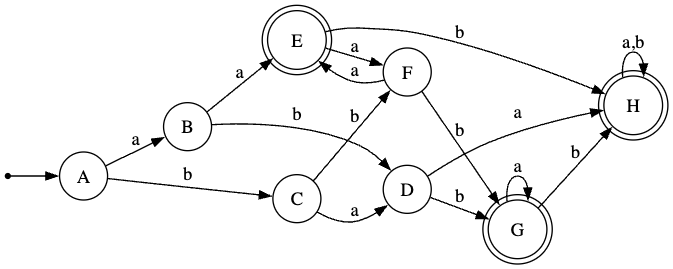
\includegraphics[width=0.7\linewidth]{images/dfa.png}
  \caption{\label{fig:dfa}Un esempio di automa a stati finiti deterministico.}
\end{figure}

\begin{table}[!htb]
  \centering
  \begin{tabular}{r|c|c}
    \toprule
                      & $a$ & $b$ \\
    \midrule
    $\rightarrow A$   & $B$ & $C$ \\
    $B$               & $E$ & $D$ \\
    $C$               & $D$ & $F$ \\
    $D$               & $H$ & $G$ \\
    $*E$              & $F$ & $H$ \\
    $F$               & $E$ & $G$ \\
    $*G$              & $G$ & $H$ \\
    $*H$              & $H$ & $H$ \\
    \bottomrule
  \end{tabular}
  \caption{\label{tab:transitions}Tabella di transizione dell'automa in Figura \ref{fig:dfa}.}
\end{table}

\section{Minimizzazione di DFA}
\label{min-dfa}

Uno dei problemi di maggiore interesse nel campo della teoria degli automi è quello riguardante la minimizzazione di 
automi a stati finiti deterministici. Il problema consiste, dato un automa $A = (Q, \Sigma, \delta, q_I, F)$,
nel trovare un automa $A' = (Q', \Sigma, \delta', q_I', F')$ tale che $L(A') = L(A)$ e $||Q'||$ sia minimo.

Il concetto alla base della minimizzazione è quello di equivalenza tra stati:

\begin{definition}
  \label{def:eq-states}
  Due stati $q_A$ e $q_B$ sono detti \emph{equivalenti}, denotato con $q_A \equiv q_B$, 
  se $\forall w \in \Sigma^*$, $\hat{\delta}(q_A, w) \in F$ se e solo se $\hat{\delta}(q_B, w) \in F$.
  Specularmente, due stati $q_A$ e $q_B$ non equivalenti sono detti distinguibili.
\end{definition}

\begin{theorem}
  \label{th:eq-rel-states}
  "$\equiv$" è una relazione di equivalenza, ovvero, è riflessiva, simmetrica e transitiva.
\end{theorem}

L'importanza dell'equivalenza tra stati è evidente nel momento in cui si considera che
due stati equivalenti, possono essere sostituiti da un singolo stato che si comporti come entrambi.
La diretta conseguenza risiede nel fatto che, dato un automa di partenza $A = (Q, \Sigma, \delta, q_I, F)$, 
siano $q_A, q_B \in Q$ tali che $q_A \equiv q_B$, è possibile costruire un automa $A' = (Q', \Sigma, \delta', q_I', F')$,
con $||Q'|| < ||Q||$ e $L(A') = L(A)$, facendo collassare gli stati $q_A$ e $q_B$ in un singolo stato $q'$, ovvero, definendo
$Q' = Q \setminus \{q_A, q_B\} \cup \{q'\}$ e la funzione di transizione $\delta'$
in modo che tutte le transizioni in ingresso a $q_A$ e $q_B$ vengano reindirizzate a $q'$ e che
$\delta'(q', \sigma) = \delta(q_A, \sigma)$ per ogni $\sigma \in \Sigma$, prestando particolare attenzione,
se necessario, anche alla conseguente ridefinizione dello stato iniziale e degli stati finali in $A'$.

Il Teorema \ref{th:eq-rel-states} permette di estendere il risultato sopra riportato ad un numero arbitrario di
stati equivalenti, più formalmente, siano $q_1, q_2, \dots, q_n \in Q$ con $n \in \mathbb{N}$ tali che
$q_1 \equiv q_2 \equiv \dots \equiv q_n$, allora è possibile collassare gli stati $q_1, q_2, \dots, q_n$ in un
singolo stato $q'$ mantenendo il linguaggio riconosciuto dall'automa inalterato.

Grazie all'idea di equivalenza tra stati, è possibile definire l'equivalenza tra automi: siano
$A_1 = (Q_1, \Sigma, \delta_1, q_{I_1}, F_1)$ e $A_2 = (Q_2, \Sigma, \delta_2, q_{I_2}, F_2)$ due DFA, 
$A_1$ è detto \emph{equivalente} ad $A_2$, denotato con $A_1 \equiv A_2$, se $q_{I_1} \equiv q_{I_2}$.
É banale osservare che, se $A_1 \equiv A_2$, questi accettano gli stessi input, pertanto $L(A_1) = L(A_2)$.

Ricordando inoltre che una classe di equivalenza è un sottoinsieme della partizione $P$ di un insieme $S$ determinata da
una relazione di equivalenza $R$ su $S$ \cite{Ros18}, si introduce il concetto di \emph{insieme quoziente},
denotato da $S \slash R$, come l'insieme delle classi di equivalenza di $R$ su $S$.

\begin{theorem}
  \label{th:min-dfa}
  Sia $A = (Q, \Sigma, \delta, q_I, F)$ un automa a stati finiti deterministico, $A$ è detto \emph{minimo}
  (o \emph{minimizzato}) se non esiste un automa $A' = (Q', \Sigma, \delta', q_I', F')$ tale che $A \equiv A'$ e $||Q'|| < ||Q||$.
\end{theorem}

Queste nozioni permettono di fornire quella che è la soluzione al problema della minimizzazione di un automa a
stati finiti deterministici.

Dato un automa $A = (Q, \Sigma, \delta, q_I, F)$, l'automa $A' = (Q', \Sigma, \delta', q_I', F')$ ottenuto, dapprima
rimuovendo gli stati irraggiungibili in $A$, e successivamente $\forall Q_i \in \partitioned{Q}{\equiv}$ collassando gli stati
in $Q_i$ in un singolo stato $q_i \in Q_i$ scelto arbitrariamente, è equivalente ad $A$ e $||Q'||$ è minimo.
$A'$ corrisponde quindi all'automa $A$ minimizzato.

\begin{theorem}
  \label{th:unique-min-dfa}
  L'automa minimo $A'$ ottenuto come descritto sopra è unico, questo significa che a meno di isomorfismi,
  non esiste un automa $A''$ tale che $A'' \equiv A'$ e $A'' \neq A'$.
\end{theorem}

Prendendo come esempio l'automa in Figura \ref{fig:dfa}, si procede alla sua minimizzazione seguendo
la procedura sopra descritta. L'automa risulta essere privo di stati irraggiungibili,
pertanto si procede da subito con il calcolo del partizionamento di $Q$ in classi di equivalenza,
che risulta essere
$\partitioned{Q}{\equiv} \ = \{ \{A\}, \{B\}, \{C\}, \{D\}, \{E\}, \{F\}, \{G, H\}\}$.
Si passa quindi al collasso degli stati, in particolare, gli unici stati equivalenti risultano essere
$G$ e $H$ che vengono sostituiti da un unico stato $G$, ottenendo l'automa in Figura \ref{fig:minified-dfa}.

In ultima istanza, si sottolinea come sia ben noto un algoritmo per la minimizzazione di automi a stati finiti deterministici, 
l'algoritmo di Hopcroft \cite{Hop71}, che permette, partendo da un DFA in ingresso, di ottenere l'automa minimo in tempo $n \cdot log(n)$.

\begin{figure}[!htb]
  \centering
  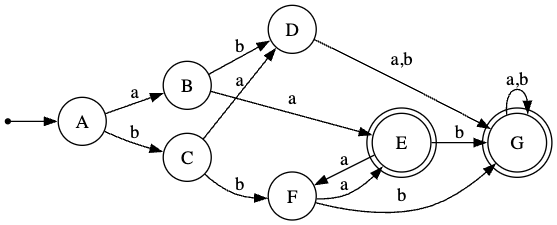
\includegraphics[width=0.7\linewidth]{images/minified-dfa.png}
  \caption{\label{fig:minified-dfa}L'automa in Figura \ref{fig:dfa} minimizzato.}
\end{figure}

% CHAPTER 2

\chapter{Iperminimizzazione di DFA}
\label{cap2}

\section{Introduzione}

Recentemente è stato introdotto un nuovo problema, affine a quello della minimizzazione, chiamato
iperminimizzazione di automi a stati finiti deterministici \cite{BGS09}.

Il problema dell'iperminimizzazione può essere visto come un'estensione del problema della minimizzazione: dove la
minimizzazione premette di ridurre al minimo il numero di stati di un DFA mantenendo inalterato il linguaggio
riconosciuto, l'imperminimizzazione prevede un'ulteriore riduzione al minimo numero di stati mantenendo invece
finita la differenza simmetrica tra il linguaggio riconosciuto dall'automa originale e quello riconosciuto
dall'automa ottenuto.

\begin{definition}\label{def:f-equiv}
  Due linguaggi $L_1$ e $L_2$ sono detti \emph{finitamente equivalenti} (o \emph{f-equivalenti}), denotato con
  $L_1 \sim L_2$, se $L_1 \Delta L_2$ è un insieme finito, dove $L_1 \Delta L_2$ denota la differenza
  simmetrica tra i linguaggi.
\end{definition}

Più formalmente dunque, dato un DFA $A = (Q, \Sigma, \delta, q_I, F)$,
l'iperminimizzazione consiste nel trovare un automa $A' = (Q', \Sigma, \delta', q_I', F')$ tale
che $L(A') \sim L(A)$ e $||Q'||$ sia minimo.

\section{Classi di quasi-equivalenza}
\label{sec:aeq-classes}

Analogamente al concetto classico di minimizzazione, in cui è di centrale rilevanza l'equivalenza tra stati,
è necessario introdurre la nozione di quasi-equivalenza tra stati per poter affrontare il problema
dell'iperminimizzazione.

\begin{definition}\label{th:aeq-states}
  Due stati $q_A$ e $q_B$ sono detti \emph{quasi-equivalenti}, denotato con $q_A \sim q_B$, 
  se $\exists k \in \mathbb{N}$, con $k \ge 0$, tale che $\forall w \in \Sigma^*$ di lunghezza $|w| \ge k$,
  $\hat{\delta}(q_A, w) \in F$ se e solo se $\hat{\delta}(q_B, w) \in F$.
\end{definition}

\begin{theorem}\label{th:aeq-rel-states}
  "$\sim$" è una relazione di equivalenza, ovvero, è riflessiva, simmetrica e transitiva.
\end{theorem}

Si introduce inoltre un importante risultato relativo alla quasi-equivalenza tra stati:

\begin{lemma}\label{lem:aeq-states}
  $q_A \sim q_B \Leftrightarrow \forall \sigma \in \Sigma, \delta(q_A, \sigma) \sim \delta(q_B, \sigma)$
\end{lemma}

Risulta evidente dunque come, grazie al Teorema \ref{th:aeq-rel-states}, sia possibile partizionare l'insieme 
degli stati $Q$ di un automa a stati finiti deterministico $A = (Q, \Sigma, \delta, q_I, F)$ in classi di quasi 
equivalenza e costruire dunque l'insieme quoziente $\partitioned{Q}{\sim}$.

Nell'automa $A = (Q, \Sigma, \delta, q_I, F)$ riportato in Figura \ref{fig:minified-dfa}, ad esempio, 
partizionando l'insieme degli stati $Q$ in classi di quasi-equivalenza, si ottiene l'insieme quoziente 
$\partitioned{Q}{\sim} \ = \{ \{ A \}, \{ C \}, \{ D, G \}, \{ F, B \}, \{ E \} \}$.

Equivalentemente a quanto visto per l'equivalenza tra stati, è possibile estendere il concetto di quasi-equivalenza
tra stati agli automi: due automi $A_1 = (Q_1, \Sigma, \delta_1,\allowbreak q_{I_1}, F_1)$ e 
$A_2 = (Q_2, \Sigma, \delta_2, q_{I_2}, F_2)$ sono detti \emph{quasi-equivalenti}, denotato con $A_1 \sim A_2$,
se $q_{I_1} \sim q_{I_2}$. Si osservi come, se $A_1 \sim A_2$, allora $L(A_1) \sim L(A_2)$.

Grazie al concetto di quasi-equivalenza tra automi, è ora possibile fornire quella che è la
definizione formale di un automa a stati finiti deterministico iperminimo.

\begin{definition}\label{def:hyper-min-dfa}
  Sia $A = (Q, \Sigma, \delta, q_I, F)$ un automa a stati finiti deterministico, $A$ è detto \emph{iperminimo}
  (o \emph{iperminimizzato}) se non esiste un automa $A' = (Q', \Sigma, \delta', q_I', F')$ tale che $A \sim A'$
  e $||Q'|| < ||Q||$.
\end{definition}

\section{Stati preambolo e kernel}
\label{sec:preamble-kernel}

Dato un automa a stati finiti deterministico $A = (Q, \Sigma, \delta, q_I, F)$, è importante, come ulteriore
passo verso la risoluzione del problema dell'iperminimizzazione, distinguere le diverse tipologie di stati 
che possono essere presenti in $A$.

É possibile partizionare l'insieme degli stati $Q$ di $A$ in tre parti: l'insieme degli stati irraggiungibili $U(A)$, 
l'insieme degli stati preambolo $P(A)$ e l'insieme degli stati kernel $K(A)$.

Sorvolando sulla definizione formale degli stati irraggiungibili, ben nota e non di centrale importanza per
la trattazione, viene fornita di seguito la definizione degli stati preambolo e kernel.

\begin{definition}\label{def:preamble-state}
  Uno stato $q \in Q$ è detto \emph{stato preambolo} e dunque $q \in P(A)$, se esiste almeno una parola in 
  ingresso $w \in \Sigma^*$ tale che $\hat{\delta}(q_I, w) = q$, ma il numero di tali stringhe è finito.
  In altri termini, $q$ è raggiungibile solo da un numero finito di input a partire dallo stato iniziale.
\end{definition}

\begin{definition}\label{def:kernel-state}
  Uno stato $q \in Q$ è detto \emph{stato kernel} e dunque $q \in K(A)$, se esistono infinite parole, tutte differenti tra loro, 
  in ingresso $w \in \Sigma^*$ tali che $\hat{\delta}(q_I, w) = q$.
  In altri termini, $q$ è raggiungibile da un numero infinito di input a partire dallo stato iniziale.
\end{definition}

\begin{lemma}\label{lem:kernel-state}
  Uno stato $q_A \in Q$ è in $K(A)$ se e solo se può essere raggiunto dallo stato iniziale $q_I$ attraverso
  un cammino passante per uno stato $q_B \in Q$ tale che esiste un ciclo in $A$ che inizia e termina in $q_B$.
\end{lemma}

Nell'automa $A$ riportato in Figura \ref{fig:minified-dfa}, ad esempio, è possibile osservare come gli stati 
$A$, $B$, $C$ e $D$ siano stati preambolo mentre gli stati $F$, $G$ ed $E$ siano stati kernel, o ancora, come
$P(A) = \{ A, B, C, D \}$ e $K(A) = \{ F, G, E \}$.

Si sottolinea un'importante differenza nel parallelismo tra automa minimo ed iperminimo: l'automa iperminimo
non è necessariamente unico. Si possono trovare esempi in cui un automa minimo $A'$ con $n$ stati può essere 
sostituito da diversi automi iperminimi differenti, tutti con il medesimo numero di stati $m \le n$,
ciascuno dei quali accetta un diverso linguaggio $L$ f-equivalente a $L(A')$. Tali automi possono tuttavia
differire solo per le transizioni in uscita da uno stato preambolo e in ingresso ad uno stato kernel, per i
valori accettati dagli stati preambolo, o per gli stati iniziali. In particolare, i kernel di due automi
iperminimi quasi-equivalenti sono isomorfi secondo la definizione
classica mentre i preamboli sono isomorfi, eccetto per i valori accettati.

\begin{definition}[Isomorfismo tra kernel]\label{def:kernel-isomorphism}
  Siano $A_1 = (Q_1, \Sigma, \delta_1, q_{I_1}, F_1)$ e $A_2 = (Q_2, \Sigma, \delta_2, q_{I_2}, F_2)$ due DFA,
  $A_1$ e $A_2$ hanno kernel isomorfi, denotato $A_1 \sim_K A_2$,
  se esiste una corrispondenza biunivoca $h: K(A_1) \rightarrow K(A_2)$ tale che:
  \begin{enumerate}[label=(\alph*)]
    \item $\forall q \in K(A_1)$ e $\forall \sigma \in \Sigma$, $h(\delta_1(q, \sigma))
    = \delta_2(h(q), \sigma)$;
    \item $\forall q \in K(A_1)$, $h(q) \in F_2$ se e solo se $q \in F_1$;
  \end{enumerate}
\end{definition}

\begin{theorem}\label{th:kernel-isomorphism}
  Siano $A_1$ e $A_2$ due automi minimi quasi-equivalenti, allora i loro kernel sono isomorfi ($A_1 \sim_K A_2$).
\end{theorem}

\begin{definition}[Isomorfismo tra preamboli]\label{def:preamble-isomorphism}
  Siano $A_1 = (Q_1, \Sigma, \delta_1, q_{I_1}, F_1)$ e $A_2 = (Q_2, \Sigma, \delta_2, q_{I_2}, F_2)$ due DFA,
  $A_1$ e $A_2$ hanno preamboli isomorfi, denotato $A_1 \sim_P A_2$,
  se esiste una corrispondenza biunivoca $h: P(A_1) \rightarrow P(A_2)$ tale che 
  $\forall q_{A}, q_{B} \in P(A_1)$ e $\forall \sigma \in \Sigma$ tali che $\delta_1(q_{A}, \sigma) = q_{B}$
  si ha che $\delta_2(h(q_{A}), \sigma) = h(q_{B})$.
\end{definition}

\begin{theorem}\label{th:preamble-isomorphism}
  Siano $A_1$ e $A_2$ due automi iperminimi quasi-equivalenti, allora i loro preamboli sono isomorfi ($A_1 \sim_P A_2$).
\end{theorem}

\section{Strategia generale}
\label{sec:hyperminimization-strategy}

Grazie alle nozioni presentate nelle Sezioni \ref{sec:aeq-classes} e \ref{sec:preamble-kernel}, è possibile
presentare una strategia generale per l'iperminimizzazione di automi a stati finiti deterministici.

Dato un automa $A = (Q, \Sigma, \delta, q_I, F)$, la procedura generale per l'iperminimizzazione consiste nel:
\begin{enumerate}
  \item ottenere l'automa minimo $A' = (Q', \Sigma, \delta', q_I', F')$ minimizzando classicamente $A$
  \item identificare l'insieme degli stati preambolo $P(A')$ e degli stati kernel $K(A')$
  \item determinare le classi di quasi-equivalenza su $Q'$ e costruire l'insieme $\partitioned{Q'}{\sim}$
  \item $\forall Q_i \in \partitioned{Q'}{\sim}$ tale che $||Q_i|| > 1$ ed $\exists q_{i_1} \in Q_i$ tale che $q_{i_1} \in P(A')$:
  \begin{enumerate}
    \item se $\exists q_{i_2} \in Q_i$ tale che $q_{i_2} \in K(A')$, $\forall q \in Q_i \cap P(A')$ si collassa $q$ in $q_{i_2}$
    \item altrimenti, tutti gli stati in $Q_i \setminus \{q_{i_1}\}$ sono collassati in $q_{i_1}$
  \end{enumerate}
\end{enumerate}

L'automa $A''$ così ottenuto è l'automa iperminimo.

\begin{theorem}[Caratterizzazione di un DFA iperminimo]
  \label{th:char-hyper-min-dfa}
  Un automa a stati finiti deterministico $A = (Q, \Sigma, \delta, q_I, F)$ è iperminimo se e solo se:
  \begin{enumerate}[label=(\alph*)]
    \item $A$ è minimo
    \item non esiste una coppia di stati $q_A, q_B \in Q$ tali che $q_A \neq q_B$, $q_A \sim q_B$ e almeno uno dei due sia in $P(A)$
  \end{enumerate}
\end{theorem}

Si osservi che il primo passo della procedura, ovvero la minimizzazione dell'automa, permette di garantire 
che l'automa minimo ottenuto $A'$, sia privo di stati irraggiungibili ($U(A') = \emptyset$) e che quindi nei passaggi
successivi della strategia l'insieme degli stati possa essere partizionato
esclusivamente in due parti, gli stati preambolo e gli stati kernel ($Q' = P(A') \cup K(A')$).

Prendendo ancora una volta come esempio l'automa $A = (Q, \Sigma, \delta, q_I, F)$ in Figura \ref{fig:dfa},
si procede alla sua iperminimizzazione seguendo la strategia generale appena descritta.
La minimizzazione dell'automa, discussa in precedenza, porta all'automa minimo $A' = (Q', \Sigma, \delta', q_I', F')$
in Figura \ref{fig:minified-dfa}.
Ricordando ora che $P(A') = \{ A, B, C, D \}$, $K(A') = \{ F, G, E \}$ e che 
$\partitioned{Q'}{\sim} \ = \{ \{ A \}, \{ C \}, \{ D, G \}, \{ F, B \}, \{ E \} \}$,
si procede con il collasso degli stati:
\begin{enumerate}[label=--]
  \item essendo $D \sim G$, $D \in P(A')$ e $G \in K(A')$, si collassa $D$ in $G$
  \item essendo $F \sim B$, $B \in P(A')$ e $F \in K(A')$, si collassa $B$ in $F$
\end{enumerate}
ottenendo l'automa $A''$ iperminimo in Figura \ref{fig:hyper-minified-dfa}.

\begin{figure}[hbt!]
  \centering
  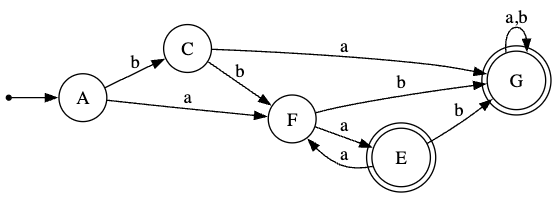
\includegraphics[width=0.7\linewidth]{images/hyper-minified-dfa.png}
  \caption{\label{fig:hyper-minified-dfa}L'automa in Figura \ref{fig:minified-dfa} iperminimizzato.}
\end{figure}

\section{Algoritmi}

Nel corso degli anni sono emersi diversi algoritmi per l'iperminimizzazione di automi a stati finiti deterministici,
ciascuno della quali, cambiando e/o raffinando le metodologie di identificazione degli stati preambolo, degli 
stati kernel e delle classi di quasi-equivalenza, e come queste siano manipolate, ha portato a differenti risultati,
migliorando la complessità temporale dei precendenti. Tutti gli algoritmi presentati di seguito condividono lo schema
ad alto livello riportato nella Sezione \ref{sec:hyperminimization-strategy} per poi specializzarsi,
in maniera differente, sulle strategie utilizzate per portare a termine le singole operazioni.

Si porta all'attenzione del lettore come, da qui in seguito, sia $A = (Q, \Sigma, \delta, q_I, F)$
l'automa in ingresso ad un algoritmo di iperminimizzazione, si utilizzerà $n$ per fare riferimento
al numero di stati $||Q||$ ed $m$ per il numero di simboli in ingresso $||\Sigma||$.

\subsection{Algoritmo di Badr, Geffert e Shipman}

L'algoritmo di Badr, Geffert e Shipman \cite{BGS09} è stato il primo algoritmo proposto per l'iperminimizzazione
in grado, dato un automa $A = (Q, \Sigma, \delta, q_I, F)$, di ottenere l'automa iperminimo 
$A'' = (Q'', \Sigma, \delta'', q_I'', F'')$ in tempo polinomiale.

Come primo passo, l'algoritmo minimizza l'automa in ingresso $A$ ottenendo l'automa minimo 
$A' = (Q', \Sigma, \delta', q_I', F')$ attraverso l'algoritmo di Hopcroft.

Successivamente, viene costruita una matrice $E$ di dimensione $||Q'|| \times ||Q'||$, utilizzata nel
passo successivo per semplificare la fase di identificazione degli insiemi $P(A')$ e $K(A')$, tale che:
\begin{equation*}
  e_{i,j} =
  \begin{cases}
    1 & \text{se } \exists w \in \Sigma^* \setminus \{ \varepsilon \} \text{ tale che } \hat{\delta}(q_i, w) = q_j \\
    0 & \text{altrimenti}
  \end{cases}
\end{equation*}

In altri termini, essendo che l'algoritmo verifica l'esistenza di un cammino di lunghezza maggiore di
1 tra ogni coppia di stati $q_i, q_j \in Q'$, trattando l'automa come un grafo, il problema può essere ricondotto 
al calcolo della chiusura transitiva di quest'ultimo. 
Sono noti diversi algoritmi per lo svolgimento di tale compito \cite{DFI08}, un possibile approccio classico potrebbe
essere quello di utilizzare l'algoritmo di Floyd-Warshall, che richiede tempo $\bigo(n^3)$, tuttavia, in questo 
caso specifico, è possibile sfruttare una ricerca in ampiezza (BFS) partendo da ogni stato $q_i \in Q'$ per
ottenere gli stati raggiungibili da $q_i$ e popolare la corrispondente riga nella matrice $E$, ottenendo
così un tempo di esecuzione $\bigo(n^2 \cdot m)$.

Ricordando ancora una volta che grazie alla minimizzazione nell'automa $A'$ non sono presenti stati irraggiungibili,
è ora possibile distinguere in $Q'$ gli stati kernel da quelli preambolo, si costruisce a questo scopo
un vettore $K$ di dimensione $||Q'||$ tale che $k_i = 1$ se e solo se $q_i \in K(A')$, altrimenti $k_i = 0$.
Grazie al Lemma \ref{lem:kernel-state} la costruzione del vettore $K$ si riduce nel determinare se per ogni
stato $q_i \in Q'$, esista uno stato $q_j \in Q'$ tale che $e_{1,j} = e_{j,j} = e_{j,i} = 1$.

É banale dunque osservare come la costruzione del vettore $K$ sia eseguita in tempo $\bigo(n)$ essendo che 
per ogni stato $q_i \in Q'$ la verifica di appartenenza a $K(A')$ richiede un tempo costante $\bigo(1)$.

L'algoritmo procede con la determinazione delle classi di quasi-equivalenza, a questo scopo, viene creato un vettore
$R$ di dimensione $||Q'||$ che conterrà in posizione $i$ l'indice $j$ della classe di quasi-equivalenza 
$Q_j \in \partitioned{Q}{\sim}$ a cui lo stato $q_i$ appartiene. 

Inizialmente, $R$ viene inizializzato in modo tale che rappresenti la partizione di $Q'$ composta esclusivamente
da singoletti $Q' = \{ q_1 \} \cup \{ q_2 \} \cup \dots \cup \{ q_{||Q'||} \}$, ovvero, 
$\forall i \in \{ 1, \dots, ||Q'|| \}, r_i = i$. 
La costruzione avviene iterativamente, si cercano coppie di stati $q_i \in Q_i$ e $q_j \in Q_j$,
con $i \neq j$, tali che $\forall \sigma \in \Sigma$ si abbia
che $\delta'(q_i, \sigma)$ e $\delta'(q_j, \sigma)$ appartengano alla stessa classe di
quasi-equivalenza $Q_l \in \partitioned{Q'}{\sim}$.
Se tale coppia di stati viene trovata, seguendo quanto riportato nel Lemma \ref{lem:aeq-states},
significa che $q_i \sim q_j$ pertanto si uniscono le classi $Q_i$ e $Q_j$ in un'unica classe e si
aggiorna il vettore $R$ di conseguenza. Il processo termina quando non vengono trovate nuove coppie
di stati che soddisfino i requisiti, il che genera al più $||Q'|| - 1$ iterazioni.

Risulta immediato stabilire che il tempo richiesto per l'inizializzazione del vettore $R$ sia lineare rispetto
al numero di stati dell'automa e che pertanto il tempo necessario a tale operazione sia $\bigo(n)$.
Necessita invece un'analisi più approfondita il calcolo della complessità temporale relativa
alla costruzione di $R$: scandire le coppie di stati in $Q'$ richiede un tempo $\bigo(n^2)$, mentre la verifica
della quasi-equivalenza per ciascuna coppia richiede un tempo $\bigo(m)$, essendo inoltre il processo iterato
al più $||Q'|| - 1$ volte, la complessità temporale totale risulta essere $\bigo(n^3 \cdot m)$.

Infine, per ottenere l'automa $A''$ iperminimo, considerando l'insieme delle classi di quasi-equivalenza
rappresentato dal vettore $R$, si processano iterativamente tutti i $Q_i \in \partitioned{Q'}{\sim}$
collassando ove possibile gli stati seguendo quanto descritto nel punto 4 della strategia generale riportata
nella Sezione \ref{sec:hyperminimization-strategy}.

Il tempo complessivo richiesto dall'algoritmo per la costruzione dell'automa
iperminimo $A''$ risulta quindi essere $\bigo(n^3 \cdot m)$.

Supponendo, a titolo di esempio, di stare iperminimizzando l'automa $A'$ in Figura \ref{fig:minified-dfa},
la matrice $E$ costruita dall'algoritmo risulterebbe essere:
\begin{center}
  $E = \begin{bNiceMatrix}[last-col, first-row]
    \scriptstyle{A} & \scriptstyle{B} & \scriptstyle{C} & \scriptstyle{D} & \scriptstyle{E} & \scriptstyle{F} & \scriptstyle{G} \\
    0 & 1 & 1 & 1 & 1 & 1 & 1 & \scriptstyle{A} \\
    0 & 0 & 0 & 1 & 1 & 1 & 1 & \scriptstyle{B} \\
    0 & 0 & 0 & 1 & 1 & 1 & 1 & \scriptstyle{C} \\
    0 & 0 & 0 & 0 & 0 & 0 & 1 & \scriptstyle{D} \\
    0 & 0 & 0 & 0 & 1 & 1 & 1 & \scriptstyle{E} \\
    0 & 0 & 0 & 0 & 1 & 1 & 1 & \scriptstyle{F} \\
    0 & 0 & 0 & 0 & 0 & 0 & 1 & \scriptstyle{G} \\
  \end{bNiceMatrix}$
\end{center}

mentre i vettori $K$ dei kernel e $R$ delle classi di quasi-equivalenza risulterebbero essere:

\begin{center}
  $K = \begin{bNiceMatrix}[last-row]
    0 & 0 & 0 & 0 & 1 & 1 & 1 \\
    \scriptstyle{A} & \scriptstyle{B} & \scriptstyle{C} & \scriptstyle{D} & \scriptstyle{E} & \scriptstyle{F} & \scriptstyle{G}
  \end{bNiceMatrix}$, 
  \
  $R = \begin{bNiceMatrix}[last-row]
    A & F & C & D & E & F & D \\
    \scriptstyle{A} & \scriptstyle{B} & \scriptstyle{C} & \scriptstyle{D} & \scriptstyle{E} & \scriptstyle{F} & \scriptstyle{G}
  \end{bNiceMatrix}$
\end{center}

\subsection{Algoritmo di Badr}

L'algoritmo proposto da Andrew Badr \cite{Badr} migliora la complessità temporale dell'algoritmo
di Badr, Geffert e Shipman cambiando quella che è la strategia utilizzata per identificare le classi di
quasi-equivalenza.

Equivalentemente all'algoritmo precedente, l'algoritmo di Badr minimizza come prima operazione l'automa
in ingresso $A$ ottenendo l'automa minimo $A' = (Q', \Sigma, \delta', q_I', F')$.

Il passo successivo prevede di identificare le classi di quasi-equivalenza, a questo scopo, si introduce
una nuova operazione tra automi a stati finiti deterministici e un importante risultato ad essa associato.

\begin{definition}
  Siano $A_1 = (Q_1, \Sigma, \delta_1, q_{I_1}, F_1)$ e $A_2 = (Q_2, \Sigma, \delta_2, q_{I_2}, F_2)$ due DFA,
  si definisce lo \emph{XOR cross product} tra $A_1$ e $A_2$, denotato con $A_1 \otimes A_2$, come l'automa 
  $A^\otimes = (Q^\otimes, \Sigma, \delta^\otimes, q_{I}^\otimes, F^\otimes)$ tale che:
  \begin{enumerate}
    \item $Q^\otimes = \{ (q_1, q_2) : q_1 \in Q_1 \wedge q_2 \in Q_2 \}$
    \item $\forall q_1 \in Q_1, \forall q_2 \in Q_2, \forall \sigma \in \Sigma : \delta^\otimes((q_1, q_2), \sigma) = (\delta_1(q_1, \sigma), \delta_2(q_2, \sigma))$
    \item $q_{I}^\otimes = (q_{I_1}, q_{I_2})$
    \item $F^\otimes = \{ (q_1, q_2) : (q_1 \in F_1) \otimes (q_2 \in F_2) \}$, con $\otimes$ operazione di XOR
  \end{enumerate}
\end{definition}

Un esempio di XOR cross product è quello tra l'automa in Figura \ref{fig:minified-dfa} e se stesso, il cui
risultato è riportato in Figura \ref{fig:dfa-xcp} e di cui, per una maggiore chiarezza, si riporta la tabella
di transizione in Tabella \ref{tab:dfa-xcp-transitions}.

\begin{definition}
  Sia $A = (Q, \Sigma, \delta, q_I, F)$ un automa a stati finiti deterministico, si estende la nozione
  di linguaggio riconosciuto da $A$ ad un generico stato $q \in Q$, denotato con $L(q)$ e definito \emph{linguaggio
  indotto} da $q$, come l'insieme $L(q) = \{ w \in \Sigma^* : \delta(q, w) \in F \}$.
\end{definition}

\begin{theorem}\label{th:cross-prod-state-aeq}
  Siano $A = (Q, \Sigma, \delta, q_I, F)$ un automa a stati finiti deterministico minimo e 
  $A^\otimes = (Q^\otimes, \Sigma, \delta^\otimes, q_{I}^\otimes, F^\otimes)$ l'automa risultante dallo 
  XOR cross product di $A$ con se stesso, allora: $\forall w \in \Sigma^*$ e $\forall (q_A, q_B) \in Q^\otimes$
  si ha $w \in L((q_A, q_B)) \Leftrightarrow \delta^\otimes((q_A, q_B), w) \in F^\otimes \Leftrightarrow 
  (\delta(q_A, w) \in F) \otimes (\delta(q_B, w) \in F)$.
  In altri termini, il linguaggio $L((q_A, q_B))$ di ogni stato nel contesto $A^\otimes$, è uguale al linguaggio
  $L(q_A) \Delta L(q_B)$ nel contesto $A$.
\end{theorem}
\begin{corollary}\label{cor:cross-prod-state-aeq-S}
  Siccome $A$ è minimo e dunque non esistono due stati $q_A, q_B \in Q$, con $q_A \neq q_B$, tali che inducano 
  il medesimo linguaggio, l'insieme degli stati $S = \{ (q, q) : q \in Q \}$ è esattamente l'insieme degli
  stati in $A^\otimes$ che inducono $L_\emptyset$.
\end{corollary}
\begin{corollary}\label{cor:cross-prod-state-aeq-states}
  Il linguaggio indotto da uno stato $(q_A, q_B) \in Q^\otimes$ è finito se e solo se $q_A \sim q_B$, pertanto, 
  l'insieme degli stati in $A^\otimes$ che inducono un linguaggio finito è la relazione di quasi-equivalenza
  sugli stati in $A$.
\end{corollary}

L'idea alla base dell'algoritmo di Badr è quella di utilizzare l'automa $A^\otimes$ prodotto dallo 
XOR cross product tra l'automa minimo $A'$ e se stesso, la cui costruzione richiede tempo $\bigo(n^2)$,
per computare $\partitioned{Q'}{\sim}$.
In particolare, l'algoritmo utilizza il sottoinsieme $R \subset Q^\otimes$ di tutti gli stati
che inducono un linguaggio finito in $A^\otimes$ per calcolare le classi di quasi-equivalenza su $Q'$.

A questo scopo si calcola l'insieme degli stati che inducono il linguaggio vuoto $S$ in $A^\otimes$ ed il suo 
insieme complementare $S^C$. Si osservi come, dato un automa a stati finiti deterministico generico 
$M = (Q_M, \Sigma_M, \delta_M, q_{I_M}, F_M)$, l'insieme degli stati che inducono un linguaggio finito in $M$
è per definizione $S_M = \{q \in Q_M \ t.c. \ \forall w \in \Sigma^*_M, \ \delta_M(q, w) \notin F_M\}$ che in
$A^\otimes$, per il Corollario \ref{cor:cross-prod-state-aeq-S}, corrisponde all'insieme $S = \{ (q, q) : q \in Q' \}$. É banale dunque osservare come la costruzione di $S$ e $S^C$
richiede un tempo $\bigo(n)$.

\begin{figure}
  \centering
  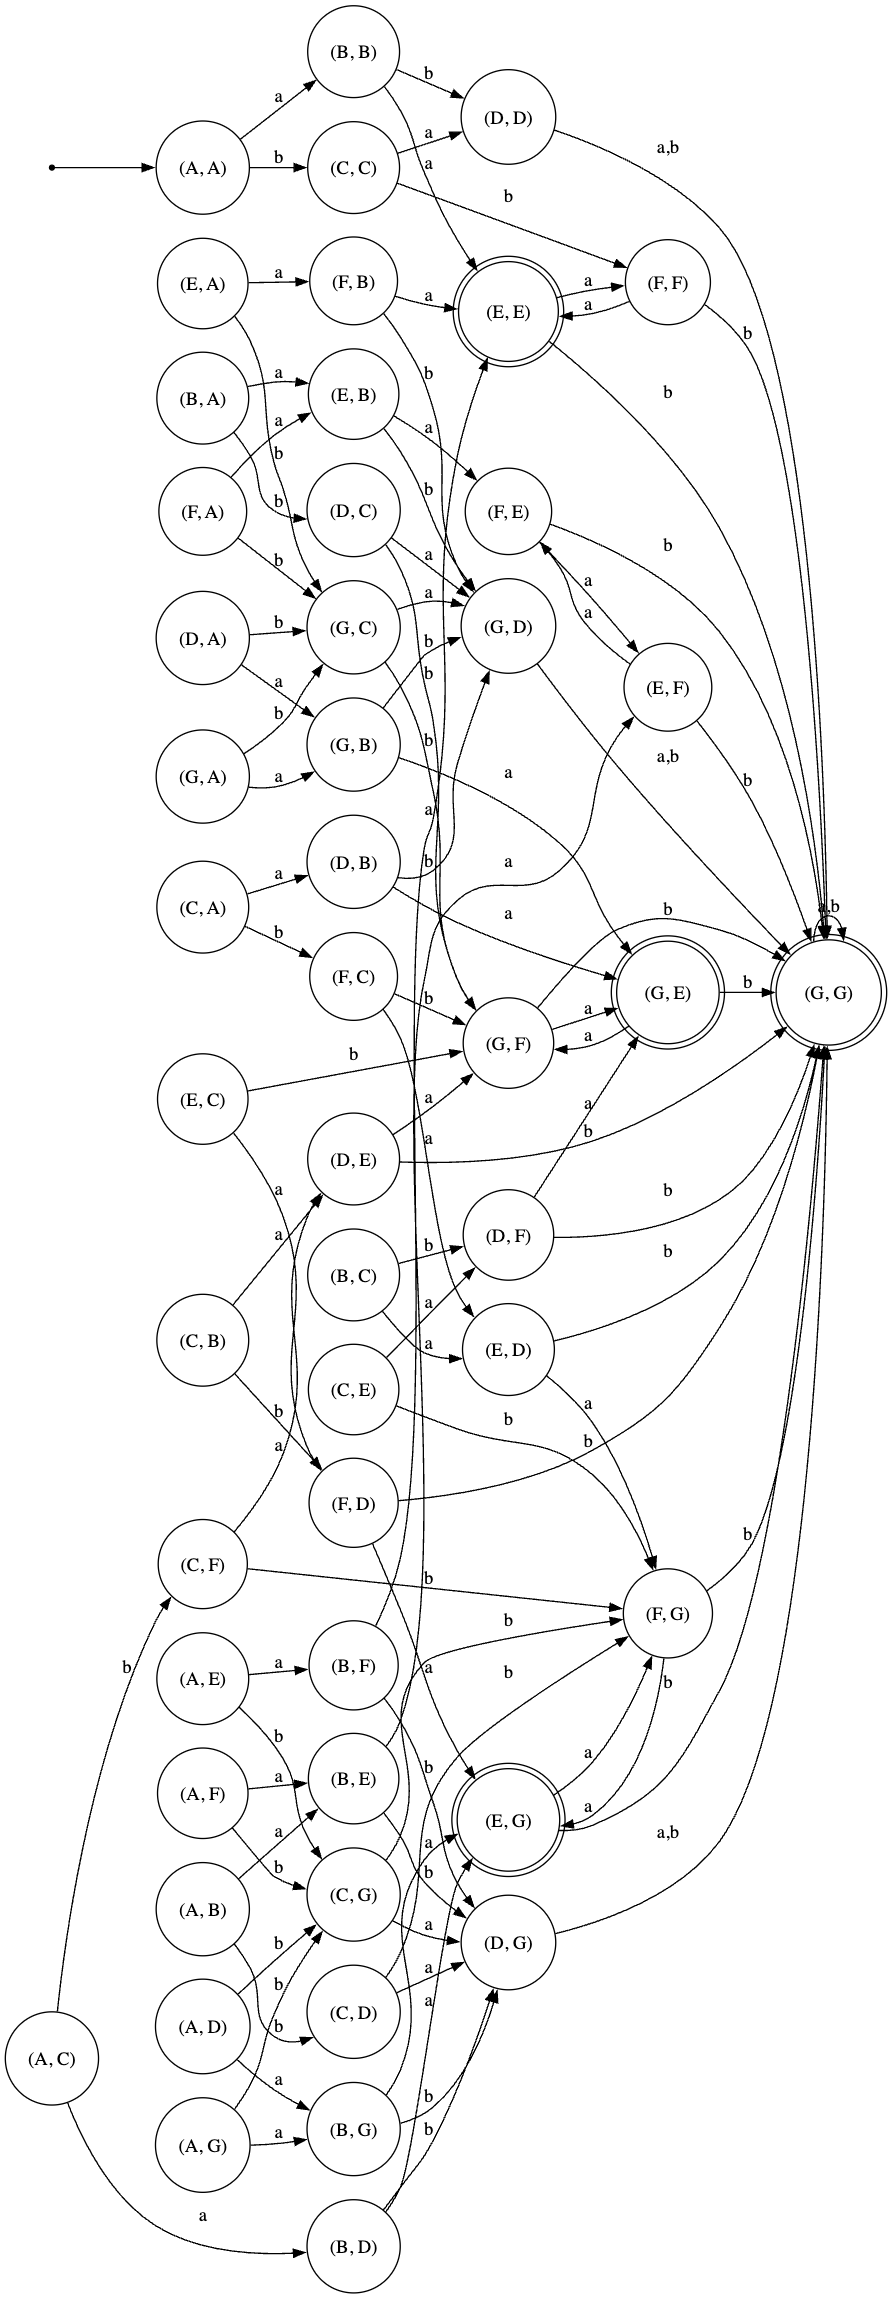
\includegraphics[width=0.5\linewidth]{images/dfa_xcp.png}
  \caption{\label{fig:dfa-xcp}L'automa in Figura \ref{fig:minified-dfa} in XOR cross product con se stesso.}
\end{figure}

\begin{table}[!htb]
  \centering
  \begin{tabular}[t]{r|c|c}
    \toprule
                          & $a$       & $b$       \\
    \midrule
    $\rightarrow (A, A)$  & $(B, B)$  & $(C, C)$  \\
    $(A, B)$              & $(B, E)$  & $(C, D)$  \\
    $(A, C)$              & $(B, D)$  & $(C, F)$  \\
    $(A, D)$              & $(B, G)$  & $(C, G)$  \\
    $(A, E)$              & $(B, F)$  & $(C, G)$  \\
    $(A, F)$              & $(B, E)$  & $(C, G)$  \\
    $(A, G)$              & $(B, G)$  & $(C, G)$  \\
    $(B, A)$              & $(E, B)$  & $(D, C)$  \\
    $(B, B)$              & $(E, E)$  & $(D, D)$  \\
    $(B, C)$              & $(E, D)$  & $(D, F)$  \\
    $(B, D)$              & $(E, G)$  & $(D, G)$  \\
    $(B, E)$              & $(E, F)$  & $(D, G)$  \\
    $(B, F)$              & $(E, E)$  & $(D, G)$  \\
    $(B, G)$              & $(E, G)$  & $(D, G)$  \\
    $(D, B)$              & $(G, E)$  & $(G, D)$  \\
    $(D, C)$              & $(G, D)$  & $(G, F)$  \\
    $(D, D)$              & $(G, G)$  & $(G, G)$  \\
    $(C, A)$              & $(D, B)$  & $(F, C)$  \\
    $(C, B)$              & $(D, E)$  & $(F, D)$  \\
    $(C, C)$              & $(D, D)$  & $(F, F)$  \\
    $(C, D)$              & $(D, G)$  & $(F, G)$  \\
    $(C, E)$              & $(D, F)$  & $(F, G)$  \\
    $(C, F)$              & $(D, E)$  & $(F, G)$  \\
    $(C, G)$              & $(D, G)$  & $(F, G)$  \\
    $(D, A)$              & $(G, B)$  & $(G, C)$  \\
    \bottomrule
  \end{tabular}
  \quad
  \begin{tabular}[t]{r|c|c}
    \toprule
              & $a$       & $b$       \\
    \midrule
    $(D, E)$  & $(G, F)$  & $(G, G)$  \\
    $(D, F)$  & $(G, E)$  & $(G, G)$  \\
    $(D, G)$  & $(G, G)$  & $(G, G)$  \\
    $(E, A)$  & $(F, B)$  & $(G, C)$  \\
    $(E, B)$  & $(F, E)$  & $(G, D)$  \\
    $(E, C)$  & $(F, D)$  & $(G, F)$  \\
    $(E, D)$  & $(F, G)$  & $(G, G)$  \\
    $*(E, E)$ & $(F, F)$  & $(G, G)$  \\
    $(E, F)$  & $(F, E)$  & $(G, G)$  \\
    $*(E, G)$ & $(F, G)$  & $(G, G)$  \\
    $(F, A)$  & $(E, B)$  & $(G, C)$  \\
    $(F, B)$  & $(E, E)$  & $(G, D)$  \\
    $(F, C)$  & $(E, D)$  & $(G, F)$  \\
    $(F, D)$  & $(E, G)$  & $(G, G)$  \\
    $(F, E)$  & $(E, F)$  & $(G, G)$  \\
    $(F, F)$  & $(E, E)$  & $(G, G)$  \\
    $(F, G)$  & $(E, G)$  & $(G, G)$  \\
    $(G, A)$  & $(G, B)$  & $(G, C)$  \\
    $(G, B)$  & $(G, E)$  & $(G, D)$  \\
    $(G, C)$  & $(G, D)$  & $(G, F)$  \\
    $(G, D)$  & $(G, G)$  & $(G, G)$  \\
    $*(G, E)$ & $(G, F)$  & $(G, G)$  \\
    $(G, F)$  & $(G, E)$  & $(G, G)$  \\
    $*(G, G)$ & $(G, G)$  & $(G, G)$  \\
    \bottomrule
  \end{tabular}
  \caption{\label{tab:dfa-xcp-transitions}Tabella di transizione dell'automa in Figura \ref{fig:dfa-xcp}.}
\end{table}

Una volta calcolati $S$ e $S^C$, l'algoritmo procede istanziando per ogni stato $q \in Q^\otimes$ due insiemi
$T^\rightarrow_q = \emptyset$ e $T^\leftarrow_q = \emptyset$ che conterranno rispettivamente gli stati raggiungibili
da $q$ e gli stati che possono raggiungere $q$. La costruzione di $T^\rightarrow_q$ e $T^\leftarrow_q$ avviene
iterativamente: per ogni stato $q \in S^C$ e per ogni $\sigma \in \Sigma$, sia $q' = \delta^\otimes(q, \sigma)$,
allora $T^\rightarrow_q = T^\rightarrow_q \cup \{ (q', \sigma) \}$ e 
$T^\leftarrow_{q'} = T^\leftarrow_{q'} \cup \{ (q, \sigma) \}$.

In seguito, viene costruito l'insieme $R$, inizializzato come $R = \emptyset$, iterativamente: fino a quando
$S \neq \emptyset$, si estrae uno stato $q \in S$ e lo si aggiunge ad $R$, si rimuove $q$ da $S$ e 
$\forall (q', \sigma) \in T_q^\leftarrow$ si rimuove $(q, \sigma)$ da $T_{q'}^\rightarrow$ e se, in seguito
a tale rimozione, $T_{q'}^\rightarrow = \emptyset$, si aggiunge $q'$ a $S$.

\begin{theorem}\label{th:rfs-correctness}
  L'algoritmo appena descritto aggiunge uno stato all'insieme $R$ se e solo se induce un linguaggio finito in $A^\otimes$.
\end{theorem}

Al termine di questo processo, grazie al risultato esposto nel Teorema \ref{th:rfs-correctness}, per la cui dimostrazione
il lettore è rimandato a \cite{Badr}, l'insieme $R$ conterrà come da obiettivo tutti gli stati che inducono
un linguaggio finito in $A^\otimes$ e sarà possibile costruire $\partitioned{Q'}{\sim}$.

Essendo il numero di transizioni lineare rispetto al numero di stati, il tempo necessario alla costruzione 
di $T^\rightarrow_q$ e $T^\leftarrow_q$ per tutti gli stati corrisponde complessivamente a $\bigo(||Q^\otimes||)$,
inoltre, l'aggiunta di ogni stato ad $R$ richiede un tempo costante $\bigo(1)$ più un tempo trascurabile per ciascuno
stato da cui si raggiunge quello corrente, pertanto la costruzione di $R$ richiede anch'essa un tempo
lineare $\bigo(||Q^\otimes||)$. Ricordando che $A^\otimes$ è lo XOR cross product di $A'$ con se stesso, la complessità
temporale di questo passaggio è $\bigo(n^2)$.

La costruzione di $\partitioned{Q'}{\sim}$ avviene ora semplicemente, utilizzando una struttura dati QuickFind $U$ con 
bilanciamento \cite{DFI08}. La struttura viene inizializzata per rappresentare la partizione
di $Q'$ composta esclusivamente da singoletti, quindi, per ogni stato $(q_A, q_B) \in R$, siano $Q_i$ e $Q_j$
rispettivamente i risultati delle operazioni di $find(q_A)$ e $find(q_B)$ in $U$, se $Q_i \neq Q_j$, 
allora si uniscono gli insiemi $Q_i$ e $Q_j$ tramite l'operazione $union(Q_i, Q_j)$ in $U$. Per il 
Corollario \ref{cor:cross-prod-state-aeq-states}, al termine dell'operazione, $U$ rappresenterà $\partitioned{Q'}{\sim}$.

Dato l'utilizzo di una struttura dati QuickFind con bilanciamento, il costo della singola operazione di $find$
è costante, mentre il costo della singola operazione di $union$ è lineare, pertanto
essendo che per la costruzione di $\partitioned{Q'}{\sim}$ vengono eseguite al più $n - 1$ operazioni di $union$ e si
cicla lungo tutti gli stati in $R$, la complessità temporale di questo passaggio è $\bigo(n^2)$.

Il calcolo degli insieme $K(A')$ e $P(A')$ avviene in tempo $\bigo(n^2)$, l'idea è simile a quella dell'algoritmo di 
Badr, Geffert e Shipman, ma in questo caso ne viene cambiata la messa in pratica. Si inizializza l'insieme 
$K = \emptyset$ che conterrà gli stati kernel e si procede iterativamente: per ogni stato $q \in Q'$ si ottiene
l'insieme degli stati raggiungibili da $q$ in $A'$ con un cammino di lunghezza maggiore di 1, se tale insieme
contiene $q$ allora si aggiunge $q$ a $K$. Al termine del processo, $K$ conterrà tutti gli stati kernel e l'insieme
$P = P(A')$ sarà dato da $Q' \setminus K$.

Infine, l'automa iperminimo $A''$ viene costruito: per ogni classe di quasi-equivalenza $Q_i \in U$,
si ottiene l'insieme $P_{Q_i}$ degli stati preambolo in $Q_i$ e l'insieme $K_{Q_i}$ degli stati kernel in $Q_i$
tramite intersezione di $Q_i$ rispettivamente con $P$ e $K$. Si procede dunque al collasso di tutti gli stati
in $P_{Q_i}$ in uno stato $q_K \in K_{Q_i}$, se $K_{Q_i}$ è non vuoto, o al collasso in 
$q_P \in P_{Q_i}$ degli stati in $P_{Q_i} \setminus \{ q_P \}$ altrimenti.

Utilizzando ancora una volta come esempio l'automa $A'$ in Figura \ref{fig:minified-dfa}, l'automa $A^\otimes$
risultante dallo XOR cross product tra $A'$ e se stesso è stato mostrato essere quello descritto in Tabella 
\ref{tab:dfa-xcp-transitions}. L'insieme $S$ degli stati che inducono un linguaggio finito in $A^\otimes$ 
ne segue essere $S = \{ (A, A), (B, B), (C, C), (D, D), (E, E), (F, F), (G, G) \}$, da cui l'insieme $R$ 
degli stati che inducono un linguaggio finito in $A'$ costruito dall'algoritmo è 
$R = S \cup \{ (B, F), (F, B), (D, G), (G, D) \}$. L'insieme delle classi di quasi-equivalenza
rappresentato da $U$ risulta correttamente essere $\{ \{ A \}, \{ B, F \}, \{ C \}, \{ D, G \}, \{ E \} \}$.

\subsection{Algoritmo di Holzer e Maletti}

L'ultimo algoritmo presentato è quello proposto da Holzer e Maletti \cite{HM10}, questo migliora i risultati
ottenuti in precedenza infatti, indroducento una nuova stategia per l'identificazione degli stati
kernel e per la costruzione delle classi di equivalenza, riduce la complessità temporale a $\bigo(n\log n)$.

Siano $A = (Q, \Sigma, \delta, q_I, F)$ un automa a stati finiti deterministico e $q_A, q_B \in Q$ due stati,
si definisce formalmente una funzione \emph{merge} utilizzata in seguito dall'algoritmo per il collasso
degli stati come $merge(\delta, q_I, q_A, q_B) = (\delta', q_I')$ tale che $\forall q' \in Q$ e
$\forall \sigma \in \Sigma$:
\begin{equation*}
  \delta'(q', \sigma) =
  \begin{cases}
    q_B                 & \text{se } \delta(q', \sigma) = q_A \\
    \delta(q', \sigma)  & \text{altrimenti}
  \end{cases}
  \text{ e } 
  q_I' =
  \begin{cases}
    q_B & \text{se } q_I = q_A \\
    q_I & \text{altrimenti}
  \end{cases}
\end{equation*}

L'algoritmo inizia seguendo quella che è la linea generale degli algoritmi precedenti: minimizza 
l'automa in ingresso ottenendo l'automa minimo $A' = (Q', \Sigma, \delta', q_I', F')$.

\begin{definition}
  Sia $A = (Q, \Sigma, \delta, q_I, F)$ un automa a stati finiti deterministico, uno stato $q \in Q$ è detto
  \emph{stato centrale} se $\exists w \in \Sigma^* \setminus \{ \varepsilon \}$ tale che $\delta(q, w) = q$.
\end{definition}

Il passo successivo prevede di identificare l'insieme $K(A')$ degli stati kernel in $A'$. L'idea alla base
della strategia utilizzata dall'algoritmo è quella di identificare l'insieme $C$ degli stati centrali in $A'$ 
attraverso una versione dell'algoritmo di Tarjan \cite{DFI08} per l'identificazione delle componenti fortemente
connesse semplificata in quanto, essendo $A'$ minimo, tutti gli stati in $Q'$ sono raggiungibili da $q_I'$. 
Questo avviene semplicemente in quanto, per definizione, gli stati centrali sono parte di una
componente fortemente connessa di almeno due stati o hanno un ciclo su loro stessi.
Una volta costruito l'insieme $C$ una Depth-First Search \cite{DFI08} viene utilizzata per identificare tutti
gli stati raggiungibili da uno stato centrale, questi stati sono gli stati kernel per il Lemma \ref{lem:kernel-state}.

L'algoritmo passa ora ad occuparsi della costruzione delle classi di quasi-equivalenza. Per ottenere una migliore
complessità temporale rispetto agli algoritmi precedenti, la strategia utilizzata prevede di evitare i confronti
tra coppie, che migliora la complessità di un fattore $\bigo(n)$, e di collassare gli stati con una metodologia 
specifica che riduce un fattore $\bigo(n)$ a $\bigo(\log n)$. 

\begin{definition}
  Sia $A = (Q, \Sigma, \delta, q_I, F)$ un automa a stati finiti deterministico, si definisce
  \emph{vettore dei successori} di $q \in Q$ il vettore $V(q) = [\delta(q, \sigma) \ | \ \sigma \in \Sigma]$.
\end{definition}

Nel dettaglio, l'algoritmo mantiene un insieme $I$ degli stati che devono essere processati e 
un insieme $P$ degli stati che sono ancora utili, entrambi inizializzati uguali a $Q'$,
una tabella hash $H$ inizialmente vuota che mappa vettori dei successori a stati,
una partizione $R$ di $Q'$ che ne rappresenta in partenza la partizione in singoletti, 
una funzione $\delta_\sim = \delta'$ e uno stato $q_{I_\sim} = q_I'$. 
A questo punto, fin tanto che $I \neq \emptyset$, iterativamente viene rimosso uno stato $q_A$ da $I$ e ne viene
calcolato $V(q_A)$, se a $V(q_A)$ non è associato alcun valore in $H$ allora si assegna a $V(q_A)$ lo stato $q_A$ in
$H$ e si prosegue con l'iterazione successiva, altrimenti, se è già associato uno stato $q_B$ a $V(q_A)$ in $H$, 
si determina lo stato tra $q_A$ e $q_B$ la cui cardinalità della parte in $R$ della quale è elemento è minore.
Supponendo che tale stato sia $q_A$, questo viene viene rimosso da $P$ trattandosi di uno stato inutile
in quanto collassato in $q_B$ nei prossimi passaggi, 
vengono aggiunti a $I$ tutti gli stati $q \in Q'$ per i quali $\exists \sigma \in \Sigma$ tale che
$\delta_\sim(q, \sigma) = q_A$, si effettua il $merge(\delta_\sim, q_{I_\sim}, q_A, q_B)$ aggiornando
con i valori restituiti la funzione di transizione $\delta_\sim$ e lo stato $q_{I_\sim}$ e 
si modifica la partizione $R$ unendo le parti in $R$ a cui appartengono $q_A$ e $q_B$. In ultima istanza, 
sempre in tale caso, si aggiorna il valore associato a $V(q_A)$ in $H$ con $q_B$.

\begin{theorem}\label{th:aeq-correctness}
  L'algoritmo appena descritto costruisce correttamente $\partitioned{Q'}{\sim}$.
\end{theorem}

\begin{theorem}
  \label{th:hm-complexity}
  Gli algoritmi descritti per l'identificazione degli stati kernel e per la costruzione di
  $\partitioned{Q'}{\sim}$ possono essere implementati in modo tale che la loro computazione richieda rispettivamente
  tempo $\bigo(m)$ e $\bigo(m \log n)$.
\end{theorem}

Le dimostrazioni dei Teoremi \ref{th:aeq-correctness} e \ref{th:hm-complexity} risultano essere particolarmente
lunghe e complesse, nonchè il fulcro del lavoro di Holzer e Maletti, pertanto sono volontariamente omesse 
nel presente elaborato ed il lettore è rimandato a \cite{HM10}.

Banalmente, l'ultimo passaggio dell'algoritmo consiste nel costruire l'automa iperminimo $A''$ a partire dai 
risultati ottenuti dai passaggi precedenti. Iterativamente, per ogni classe di equivalenza $Q_i \in R$, 
se l'intersezione tra $Q_i$ e $K(A')$ è non vuota, si sceglie arbitrariamente uno stato $q$ al suo interno,
altrimenti si sceglie un qualsiasi stato $q$ in $Q_i$, e $\forall q' \in Q_i \setminus K(A')$ si 
collassa $q'$ in $q$ e si aggiornano i valori di $\delta'$ e $q_I'$ tramite $merge(\delta', q_{I}', q, q')$
ottenendo l'automa iperminimo $A''$.

Ipotizzando di eseguire l'algoritmo sull'automa $A'$ in Figura \ref{fig:minified-dfa}, l'insieme $C$ degli stati
centrali risulta essere $C = \{ F, G, E \}$ dal quale viene correttamente identificato
l'insieme $K(A')$ degli stati kernel in $A'$ attraverso la visita in profondità. Ulteriormente, l'insieme $R$ delle
classi di quasi-equivalenza, costruito sulla tabella $H$ il cui contenuto al termine dell'algoritmo è riportato
in Tabella \ref{tab:hm-hash-table}, risulta correttamente essere $\partitioned{Q'}{\sim}$ come previsto dal Teorema
\ref{th:aeq-correctness}.

\begin{table}[!htb]
  \centering
  \begin{tabular}{r|c}
    \toprule
    Chiave & Valore  \\
    \midrule
    $[B, C]$  & $A$  \\
    $[D, F]$  & $C$  \\
    $[G, G]$  & $D$  \\
    $[E, G]$  & $F$  \\
    $[E, D]$  & $B$  \\
    $[F, D]$  & $E$  \\
    $[B, D]$  & $E$  \\
    $[D, D]$  & $D$  \\
    $[D, B]$  & $C$  \\
    \bottomrule
  \end{tabular}
  \caption{\label{tab:hm-hash-table}Tabella hash $H$ al termine dell'esecuzione dell'algoritmo\\sull'automa in Figura \ref{fig:minified-dfa}.}
\end{table}


% HASH {
%   (frozenset({'B'}), frozenset({'C'})): frozenset({'A'}), 
%   (frozenset({'D'}), frozenset({'F'})): frozenset({'C'}), 
%   (frozenset({'G'}), frozenset({'G'})): frozenset({'D'}), 
%   (frozenset({'E'}), frozenset({'G'})): frozenset({'F'}), 
%   (frozenset({'E'}), frozenset({'D'})): frozenset({'B'}), 
%   (frozenset({'F'}), frozenset({'D'})): frozenset({'E'}), 
%   (frozenset({'B'}), frozenset({'D'})): frozenset({'E'}), 
%   (frozenset({'D'}), frozenset({'D'})): frozenset({'D'}), 
%   (frozenset({'D'}), frozenset({'B'})): frozenset({'C'})
% }
% center {F, G, E}

% preamble {A, B, C, D}
% kernel {F, G, E}
% equivalence [{A}, {C}, {D, G}, {F, B}, {E}]

\chapter{Risultati sperimentali}

\section{Implementazione}

\subsection{Scelte implementativa}

\subsection{Strutture comuni}

\subsection{Algoritmo di Badr, Geffert e Shipman}

\subsection{Algoritmo di Badr}

\subsection{Algoritmo di Holzer e Maletti}

\section{Generazione del campione}

\subsection{Problema}

\subsection{Tecnica}

\section{Risultati}

% \begin{figure}[hbt!]
%   \centering
%   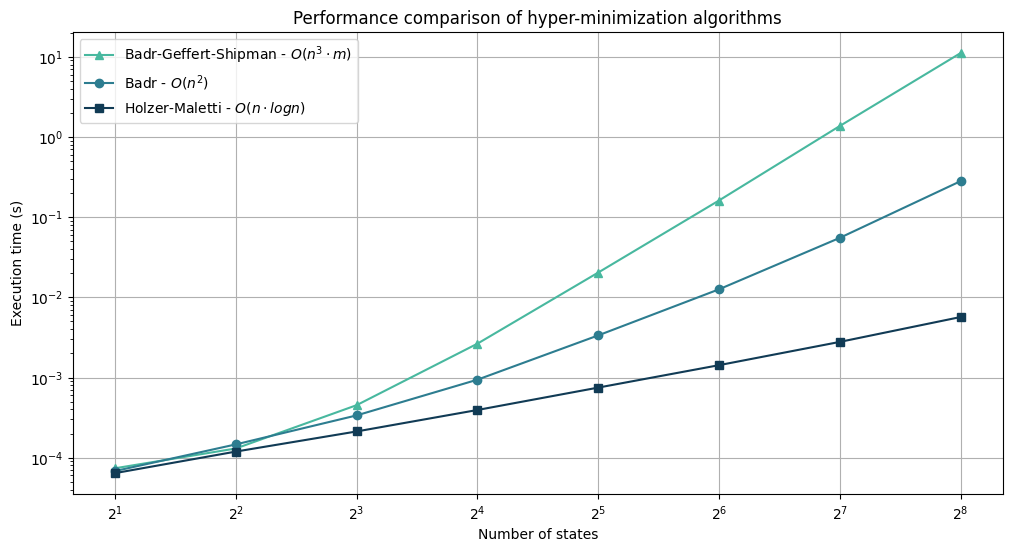
\includegraphics[width=1\linewidth]{images/performance-comparison-line.png}
%   \caption{\label{fig:performance-comparison-line}L'automa in Figura \ref{fig:xcp_start} in XOR cross product con se stesso.}
% \end{figure}
% 
% \begin{figure}[hbt!]
%   \centering
%   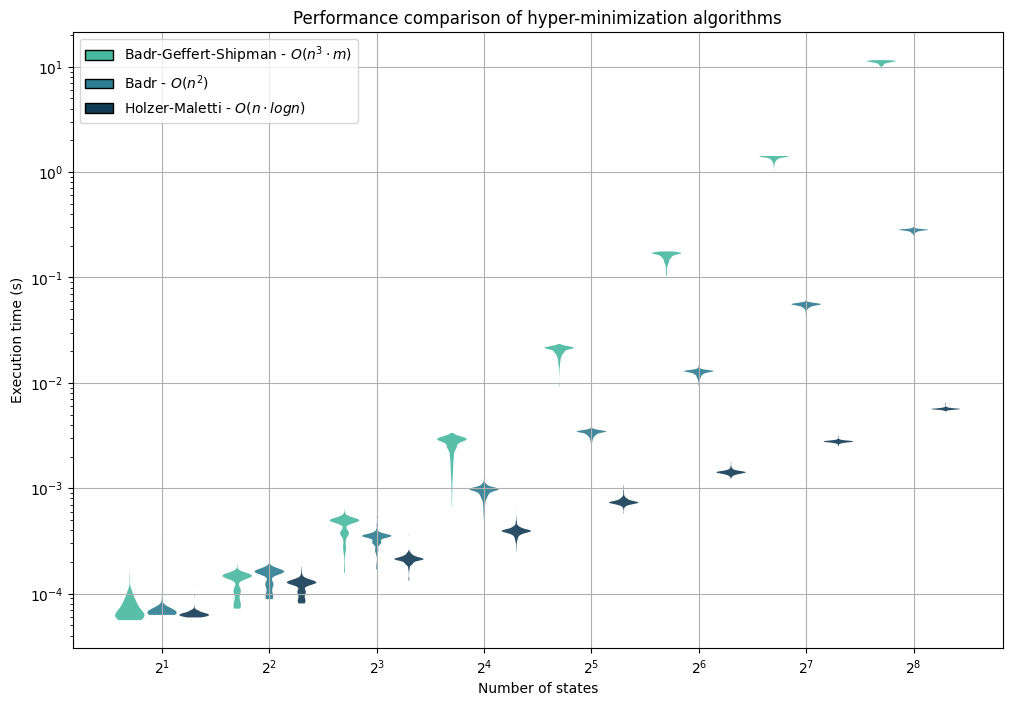
\includegraphics[width=1\linewidth]{images/performance-comparison-violin.png}
%   \caption{\label{fig:performance-comparison-violin}L'automa in Figura \ref{fig:xcp_start} in XOR cross product con se stesso.}
% \end{figure}
% 
% preamble {frozenset({'A'}), frozenset({'B'}), frozenset({'C'}), frozenset({'D'})}
% kernel {frozenset({'F'}), frozenset({'G'}), frozenset({'E'})}
% equivalence [{frozenset({'A'})}, {frozenset({'C'})}, {frozenset({'D'}), frozenset({'G'})}, {frozenset({'F'}), frozenset({'B'})}, {frozenset({'E'})}]

% è dunque chiaro che, uno stato preambolo nella medesima classe di quasi equivalenza,
% può essere collassato in uno stato kernel o preambolo

% {
%   A: {C, F, E, D, B, G}, 
%   C: {F, D, G, E}, 
%   D: {G}, 
%   F: {F, G, E}, 
%   B: {F, D, G, E},
%   G: {G}, 
%   E: {F, G, E}
% }

% \begin{algo}
%   {Algoritmo di Badr, Geffert e Shipman}
%   {Un automa a stati finiti deterministico $A = (Q, \Sigma, \delta, q_I, F)$}
%   {Uno dei possibili automi iperminimi quasi-equivalenti ad $A$}
%   $A' \gets minimize(A)$\;
%   $E \gets \text{matrice di zeri di dimensione } ||Q'|| \times ||Q'||$\;
% 
%   
% 
%   \For{$i \gets 1$ \KwTo $||Q'||$}{
%     \For{$j \gets 1$ \KwTo $||Q'||$}{
%       \If{$q_i \neq q_j$}{
%         $E[i,j] \gets 1$\;
%       }
%     }
%   }
% \end{algo}
% 

% Come visto nella sezione \ref{min-dfa}
% 
% \section{Definizione del problema}
% 
% \section{Tecniche di iperminimizzazione}

% CHAPTER 3

% SKELETON

% \chapter{Implementazione delle tecniche di iperminimizzazione}
% \label{cap3}
% 
% \section{Scelte implementative}
% 
% \section{Strutture comuni}
% 
% \section{Algoritmo di Badr, Geffert e Shipman}
% 
% \section{Algoritmo di Badr}
% 
% \section{Algoritmo di Holzer e Maletti}

% CHAPTER 4

% SKELETON

% \chapter{Risultati sperimentali}
% \label{cap4}
% 
% \section{Generazione di DFA}
% 
% \section{Risultati}

% BIBLIOGRAPHY

\bibliographystyle{alpha}
\bibliography{bibliography}

\end{document}